\hypertarget{obsah-kurzu}{%
\chapter{Obsah kurzu}\label{obsah-kurzu}}

V~poslední kapitole si představíme vytvořený online kurz pro výuku datové analytiky. Tuto část dělíme do tří vzájemně provázaných částí, z~nichž každá reflektuje odlišnou oblast návrhu a~implementace online kurzu.

\hypertarget{prux16fchod}{%
\section{Průchod}\label{prux16fchod}}

V~první částí se zaměříme na obecný průchod kurzem -- popíšeme si, jak je kurz navržen po strukturální stránce a~jakým způsobem student prochází jednotlivými částmi.

Hlavní část kurzu je tvořena sedmi hlavními obsahovými bloky, z~nichž se každý zabývá jedním určitým tématem, které na sebe přímo navazují a~představují tak hrubou strukturu online kurzu (viz Obrázek \ref{digi-bloky}). Mimo tyto ústřední bloky e-learning na začátku obsahuje úvodní text, jehož cílem je studenta navnadit ke studiu a~v~co největší stručnosti popsat obsah celého kurzu. Zároveň je pod touto úvodní kartou umístěn malý ukazatel progresu s~počtem splněných aktivit (viz další odstavec) spolu s~podkartou \emph{Užitečný tip}, která slouží v~rámci ekosystému kurzů Digiskills k~nasměrování na integrovaného chatbota (viz Obrázek \ref{digi-uvod}).

\begin{figure}[ht]   
    \centering
    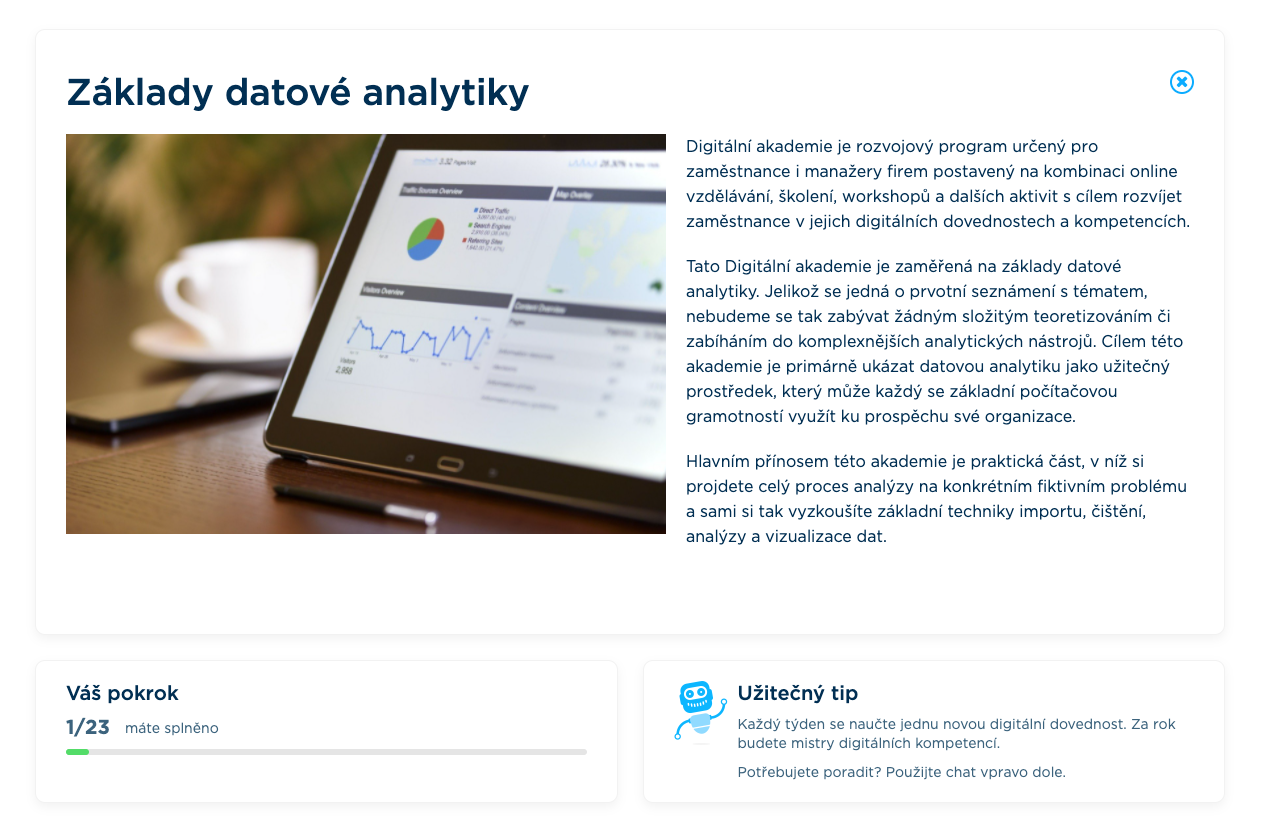
\includegraphics[width=\textwidth]{digi-uvod}  
    \caption{Úvodní obrazovka s~představením kurzu spolu s~ukazatelem progresu a~podkartou Užitečný tip}
    \label{digi-uvod}
\end{figure}

Základní jednotkou kurzu jsou pak již zmíněné aktivity, jež jsou vždy zanořeny do daného obsahového bloku (viz Obrázek \ref{digi-blok}). Těchto aktivit je v~celém kurzu v~současné chvíli 23 a~jsou do jednotlivých bloků logicky uspořádány dle následující šablony:

\begin{itemize}
\tightlist
\item
  úvodní aktivita, která uvádí studenta do daného tématu a~kontextualizuje jej v~rámci aktivit minulých a~případně následujících;
\item
  1--3 aktivity zpracovávající část tématu prostřednictvím některé z~vybraných edukačních komponent;
\item
  1--2 závěrečné aktivity, jež shrnují dané téma a~pobízí studenta k~vlastní práci ať už prostřednictvím kvízů či praktických úkolů (viz Obrázek \ref{digi-aktivity}).
\end{itemize}

\begin{figure}[ht]   
    \centering
    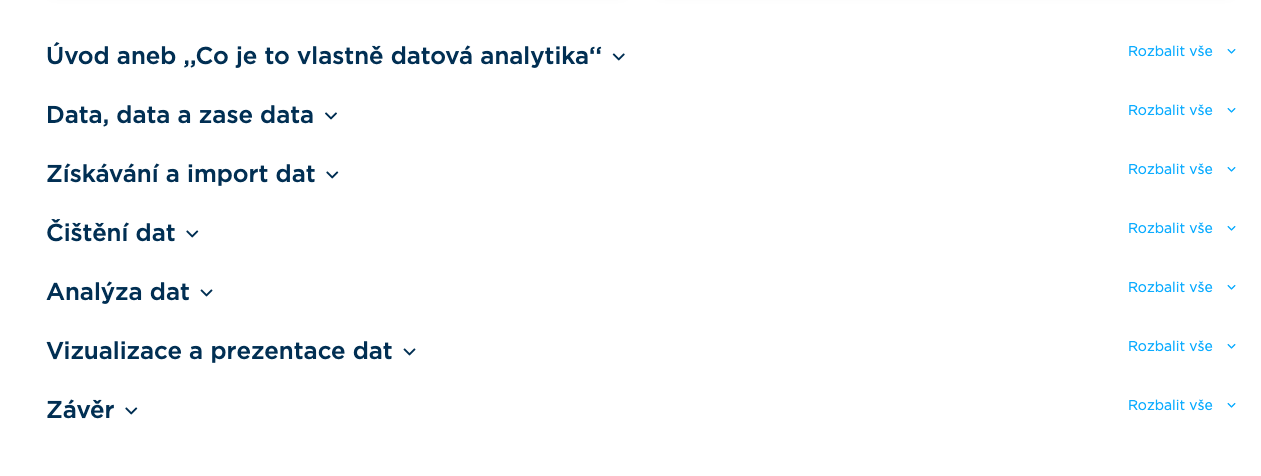
\includegraphics[width=\textwidth]{digi-bloky}  
    \caption{Nerozbalený výčet všech obsahových bloků}
    \label{digi-bloky}
\end{figure}

\begin{figure}[ht]   
    \centering
    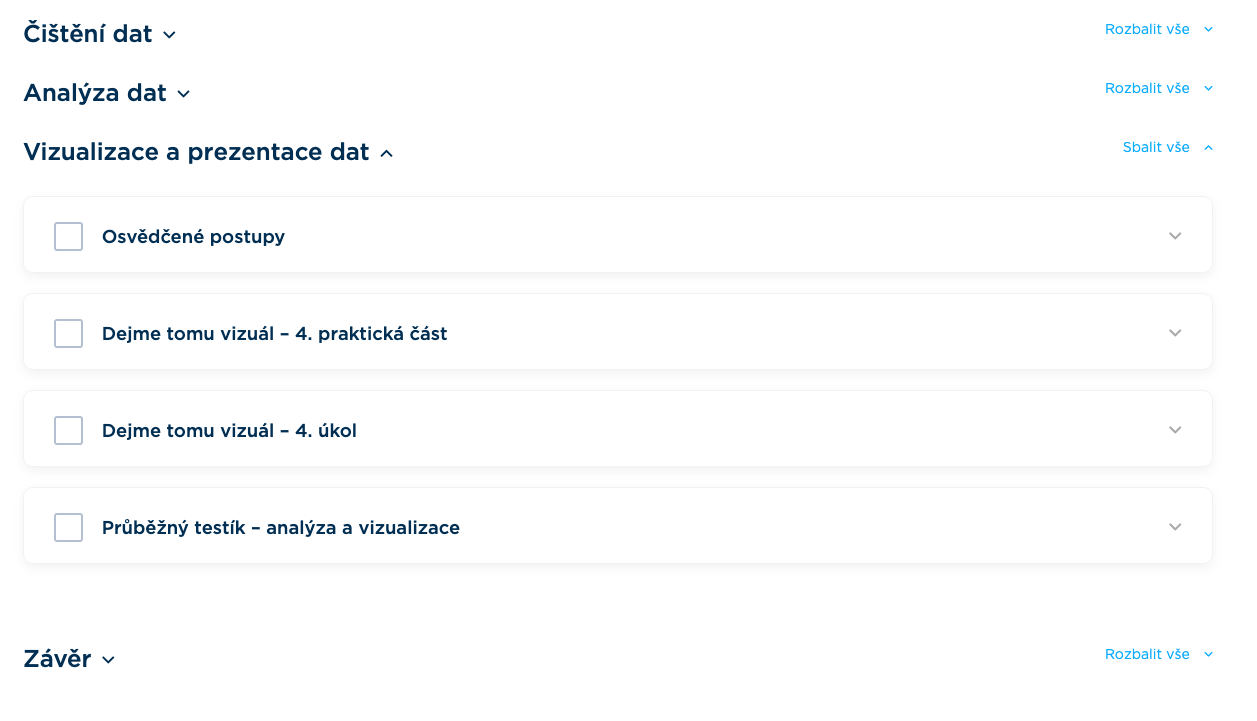
\includegraphics[width=\textwidth]{digi-blok}  
    \caption{Vnořené aktivity vztahující se ke obsahovému bloku Vizualizace a~prezentace dat}
    \label{digi-blok}
\end{figure}

\begin{figure}[ht]   
    \centering
    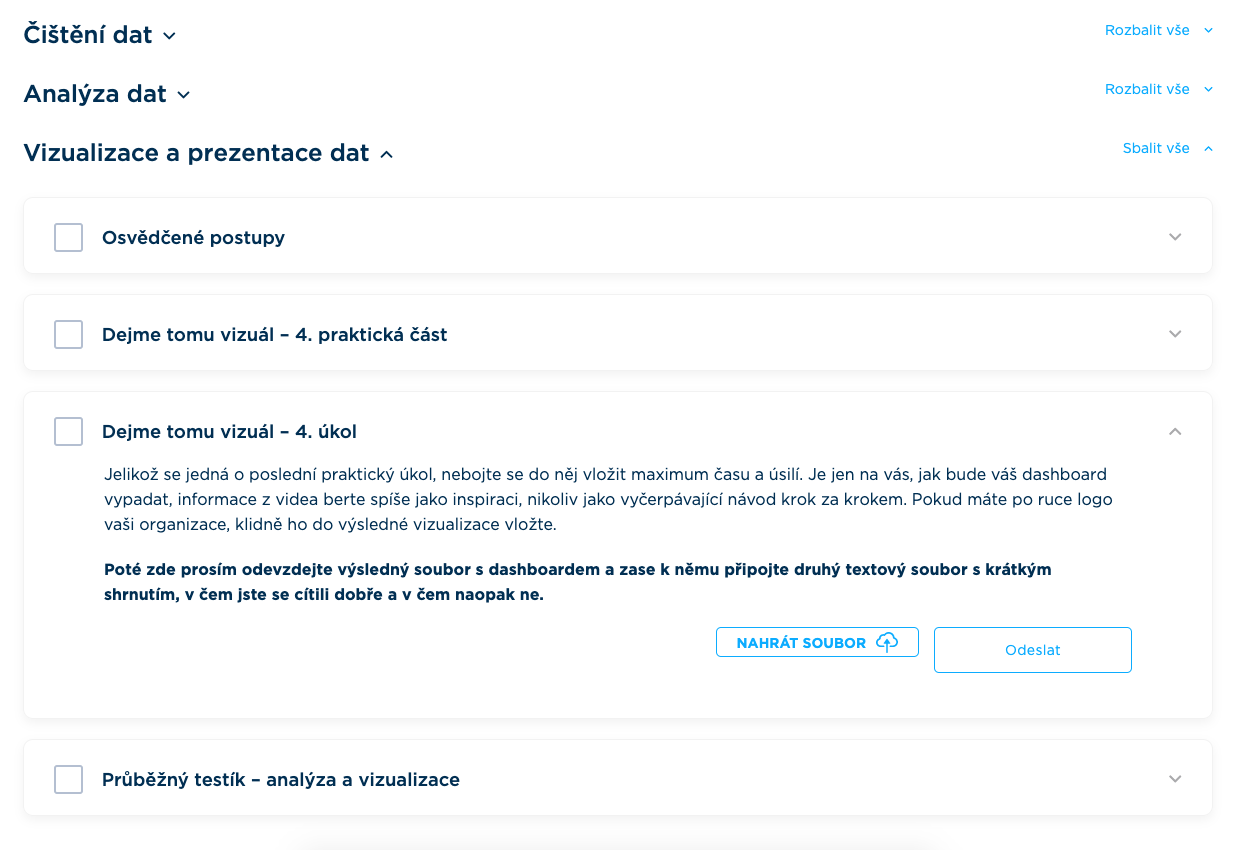
\includegraphics[width=\textwidth]{digi-aktivity}  
    \caption{Závěrečná aktivita, která obsahuje zadání praktického úkolu}
    \label{digi-aktivity}
\end{figure}

\hypertarget{komponenty}{%
\section{Komponenty}\label{komponenty}}

\hypertarget{moduly}{%
\section{Moduly}\label{moduly}}
